\subsection{Algorithm for optimising hierarchical task allocation in networks of agents}

The \acronymWSNOptimisationExtended{}{} algorithm is defined in Algorithms \ref{alg:wsn_optimisation_sink}
and \ref{alg:wsn_optimisation_arc}, which are split for clarity. The flowchart in Figure \ref{fig:algorithm-flow} shows how this agents utilise \acronymATARIA{}{} and \acronymMGRAO{}{} with these recursive actions enabled. 
\begin{figure}[ht]
	\centering
	\begin{subfigure}{.49\textwidth}
		\centering
		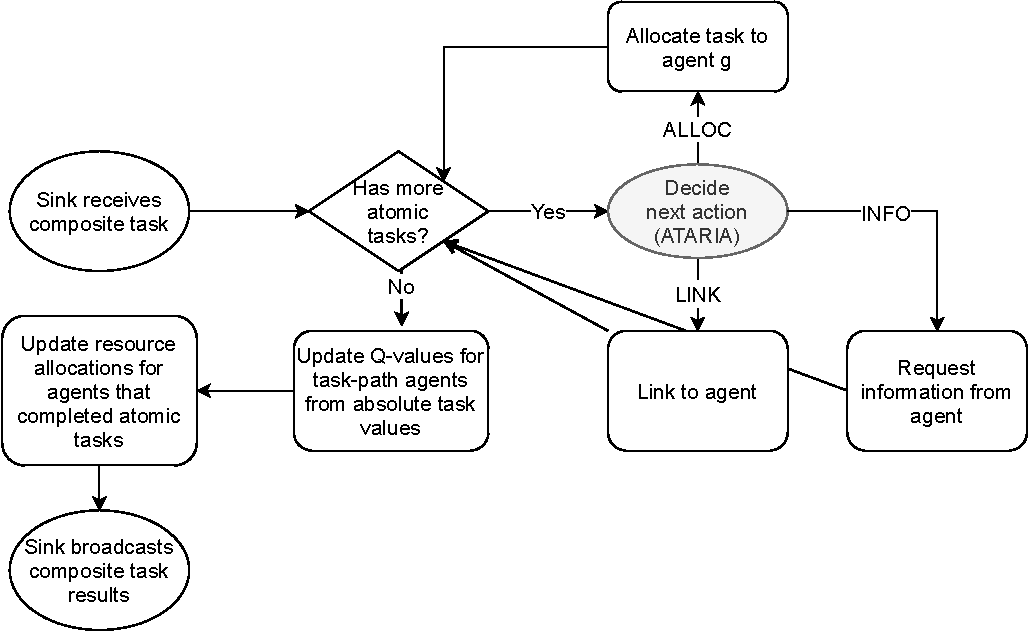
\includegraphics[width=0.9\linewidth]{algorithm-flow-sink}
		\caption{Sink agent flow}
		\label{fig:algorithm-flow-sink}
	\end{subfigure}
	\begin{subfigure}{.49\textwidth}
		\centering	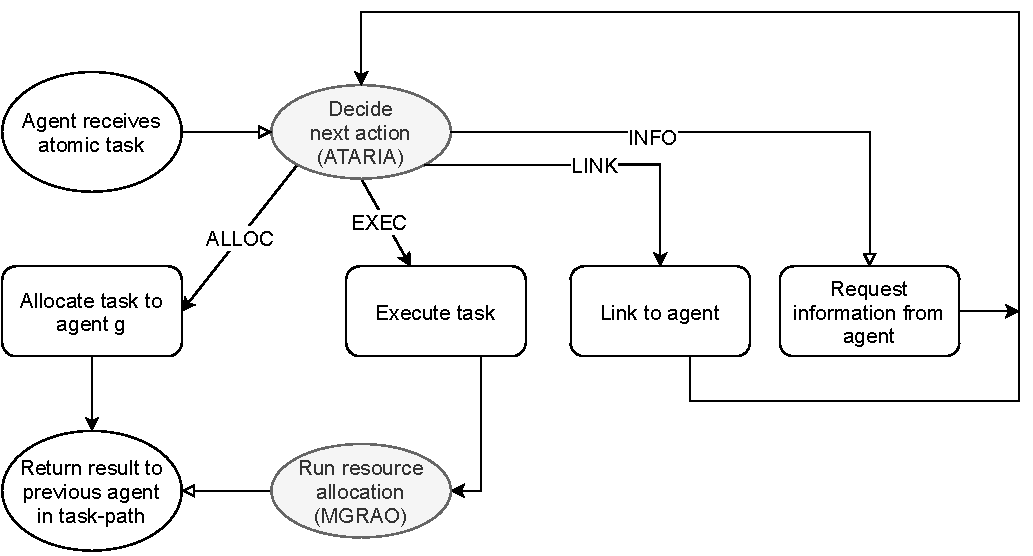
\includegraphics[width=0.9\linewidth]{algorithm-flow-arc}
		\caption{Arc agent flow}
		\label{fig:algorithm-flow-arc}
	\end{subfigure}
	\caption{\textbf{\acronymWSNOptimisation{}{}} - Flow chart of combined \acronymATARIA{}{}/\acronymMGRAO{}{} execution. The two algorithms are combined together to allow recursive allocation of tasks and learning of the network.}
	\label{fig:algorithm-flow}
\end{figure}
We formally define the \acronymWSNOptimisation{}{} algorithm in two parts, Algorithm \ref{alg:wsn_optimisation_sink} for sink agents receiving composite tasks, and Algorithm \ref{alg:wsn_optimisation_arc} for other agents that form the arc for a task.

In the \acronymWSNOptimisationSink{}{} algorithm, Algorithm \ref{alg:wsn_optimisation_sink}, the sink agent receives a composite task $\varCompositeTask{}{}$ comprising of multiple atomic tasks $\varAtomicTask{}{}$ to be completed. For each of these atomic tasks the sink agent runs the \acronymATARIA{}{} algorithm to select an action (Line \ref{wsnsink:select}). It can execute the atomic task itself (Line \ref{wsnsink:exec}), or allocate it to another agent it knows about to complete (Line \ref{wsnsink:alloc}), in both cases receiving an atomic task quality value of $\functionAtomicTaskQualitySignature{}{}$. If the action selected is one of $\functionInfo{}{}$ or $\functionLink{}{}$, those actions are carried out without any task executions. Once all atomic tasks have completed, the algorithm can then calculate each atomic tasks' proportional value to the composite task  and run the \acronymMGRAO{}{}-update algorithm on the last agent in the arc of that atomic task (Lines \ref{wsnsink:arc_last} and \ref{wsnsink:mgrao}). If the action selected is $\functionAlloc{}{}$, then the agent that has been allocated the task will enact the \acronymWSNOptimisationArc{}{} algorithm.

\newcommand{\nosemic}{\renewcommand{\@endalgocfline}{\relax}}% Drop semi-colon ;
\newcommand{\dosemic}{\renewcommand{\@endalgocfline}{\algocf@endline}}% Reinstate semi-colon ;
\newcommand{\pushline}{\Indp}% Indent
\newcommand{\popline}{\Indm\dosemic}% Undent
\let\oldnl\nl% Store \nl in \oldnl
\newcommand{\nonl}{\renewcommand{\nl}{\let\nl\oldnl}}% Remove line number for one line
\begin{algorithm}[ht]
	\DontPrintSemicolon
	\footnotesize
	
	\caption{\textbf{The \acronymWSNOptimisationSink{}{} algorithm}}
	\label{alg:wsn_optimisation_sink}
	{
		\KwIn{ $\varCompositeTask{}{}$ , The composite task set}
		\KwResult{$\functionCompositeTaskQuality{}{}{}{}$ , The composite task quality of $\varCompositeTask{}{}$}		\nonl \;

		\For{$\varAtomicTask{}{} \in \varCompositeTask{}{}$\label{wsnsink:composite_tasks}}
		{
			\tcp{Select action through \acronymATARIA{}{}}
			$\varAction{}{} \leftarrow \functionATARIA{}{}$ \label{wsnsink:select} \;	
			\uIf{$\varAction{}{} = \functionExec{}{}$?}
			{
				\tcp{Execute task $\varAtomicTask{}{}$ and get an atomic task quality} 
				$\functionAtomicTaskQualitySignature{}{} \leftarrow \functionExec{}{}$ \label{wsnsink:exec}\;
			}
			\uElseIf{$\varAction{}{} = \functionAlloc{}{}$?}{
				\tcp{allocate task $\varAtomicTask{}{}$ to agent $\varAgent{}{}$}
				$\functionAtomicTaskQualitySignature{}{} \leftarrow \functionAlloc{}{}$\label{wsnsink:alloc} \;
			}
			\uElseIf{$\varAction{}{} = \functionInfo{}{}$?}{
				\tcp{request information on system agents from agent $\varAgent{}{}$}
				$\functionInfo{}{}$ \label{wsnsink:info}\;
			}
			\uElseIf{$\varAction{}{} = \functionLink{}{}$?}{
				\tcp{allocate resources to information on to agent $\varAgent{}{}$ and maintaining network connection}
				$\functionLink{}{}$ \label{wsnsink:link}\;
			}
		}
		\For{$\varAtomicTask{}{} \in \varCompositeTask{}{}$\label{ataria:composite_tasks}}
		{
			\tcp{Target update at the last agent in the arc, the agent that completed the atomic task}
			$\varAgent{}{} \leftarrow \functionSenseRole{}{}$ \label{wsnsink:arc_last}\;
			\tcp{Run MGROA update for target agent using each atomic tasks value}
			$\functionMGRAOUpdate{}{}$ \label{wsnsink:mgrao}\;	
		}
		\Return{$\functionCompositeTaskQuality{}{}{}{}$}
	}
\end{algorithm}

The \acronymWSNOptimisationArc{}{} algorithm (Algorithm \ref{alg:wsn_optimisation_arc}) will attempt to complete an atomic task and return its quality, either by executing the task itself, or re-allocating to another agent. Using an argument $\epsilon$ as an exploration factor, a random number $[0,1]$ is generated (Line \ref{wsnarc:random}). If it is less than $\epsilon$, the \acronymATARIA{}{} algorithm is run (Line \ref{wsnarc:select}). Otherwise, the agent will attempt to complete the task and return an atomic task quality (Line \ref{wsnarc:exec}).
\begin{algorithm}[ht]
	\DontPrintSemicolon
	\footnotesize
	
	\caption{\textbf{The \acronymWSNOptimisationArc{}{} algorithm } }
	\label{alg:wsn_optimisation_arc}
	{
		\KwIn{ $\varAtomicTask{}{}$ , The atomic task to be completed}
		\KwIn{$\epsilon$, The arc exploration factor $[0,1]$.}	
		\KwResult{$\functionAtomicTaskQualitySignature{}{}$ , The atomic task quality of $\varAtomicTask{}{}$}
		\nonl \;

		\uIf{$random() < \epsilon$?\label{wsnarc:random}}
		{
			\tcp{Select an allocation action through \acronymATARIA{}{}}
			$\functionAlloc{}{} \leftarrow \functionATARIA{}{}$\label{wsnarc:select}\;	
			\tcp{allocate task $\varAtomicTask{}{}$ to agent $\varAgent{}{}$}
			$\functionAtomicTaskQualitySignature{}{} \leftarrow \functionAlloc{}{}$ \label{wsnarc:alloc}\;
		}
		\uElse{
			\tcp{execute task $\varAtomicTask{}{}$}
			$\functionAtomicTaskQualitySignature{}{} \leftarrow \functionExec{}{}$ \label{wsnarc:exec}\;
		}
	\Return{$\functionAtomicTaskQualitySignature{}{}$\label{wsnarc:return}} \;
	}
\end{algorithm}
